\documentclass{article}
\usepackage{textcomp}
\usepackage[utf8]{inputenc}
\usepackage[english]{babel}
\usepackage{gensymb}
\usepackage{float}
\usepackage{hyperref}
\hypersetup{
    colorlinks=true,
    linkcolor=blue,
    filecolor=magenta,      
    urlcolor=blue,
}
 
\urlstyle{same}
\usepackage{graphicx}
\graphicspath{ {./images/} }

\title{Physical Growth of Urban Areas in Bangladesh}
\date{2019\\ 17 April}
\author{Sakib Sadman Shajib\\ 173 1201 042\\ ENV203.1 Spring'19}


\begin{document}
\begin{titlepage}
\centering
	
\includegraphics[width=0.15\textwidth]{nsulogo}\par\vspace{1cm}
	{\scshape\LARGE North South University \par}
	\vspace{1cm}
	{\scshape\Large ENV 203: Introduction to Bangladesh Geography\par}
	\vspace{1.5cm}
	{\huge\bfseries Physical Growth of Urban Areas in Bangladesh\par}
	\vspace{2cm}
	{\Large\itshape Sakib Sadman Shajib\\ 173 1201 042\\ ENV203.1 Spring'19\par}
	\vfill
	Supervised by\par
	Dr. Saiful Momen

	\vfill

% Bottom of the page
	{\large \today\par}
\end{titlepage}
\section{Introduction}
Bangladesh is one of the fastest growing countries in the Asian continent, which makes it important to keep track of the growth of the urban areas of the country. This report is based on a research I did to calculate the growth of the three urban areas, \textit{Comilla Sadaar Dakshin (South), Mundumala (Tanore) and Hatiya}, during 2011 in compared to 2001.

I used Google Earth Engine to collect and process the data. I utilized \textit{Google USGS Landsat 5\textsuperscript{TM}} and \textit{Google USGS Landsat 7\textsuperscript{TM}} to collect the satellite images.
\section{Procedure}
The program I used, \href{https://code.earthengine.google.com/}{Google Earth Engine} is versatile piece of software provided by Google for free (until used for commercial purpose). The template script was provided by my teacher which was to be edited to suit our purpose. The script was written in JS which utilized the custom modules of the program.

Initially, I used Landsat 5 images and trained the program by drawing builtup and nonbuiltup polygons using our mouse. I had to make sure the images I am using any cloud coverage, unless the data won't be perfect. The images provided by the satellite had a resolution of 30 meter per pixel. Landsat 5 have 7 bands which was used to get more accurate data from the images. Although, I couldn't get a satellite image of \textbf{Hatiya}.

I have personally experiment with Landsat 7 satellite images, but all the images from the satellite has blank stripes on them, where there is no image data. But as \textit{Hatiya} didn't have Landsat 5 images, so I had to use the incomplete image from Landsat 7.

After everything is configured, I had to put my name, name of the location, and latitude and longitude of the two extremities of square.

\section{Comilla Sadaar Dakshin}
Comilla Sadaar Dakshin, non-existent, used to be the south Pouroshova of Comilla Sadaar. The left extremity of the urban area is 23.43\degree N and 91.12\degree E and the right extremity is 23.43\degree N, 91.25\degree E.

The result obtained by the program using \textsf{Landsat 5} are given below:

\textbf{DATA FROM 2001:}

\textsc{Builtup Area: } \textit{0.4534 sq.km.}

\textsc{Non-Builtup Area: } \textit{205.6296 sq.km.}

\textsc{Total Area: } \textit{206.0830 sq.km.}

\begin{figure}[H]
\centering
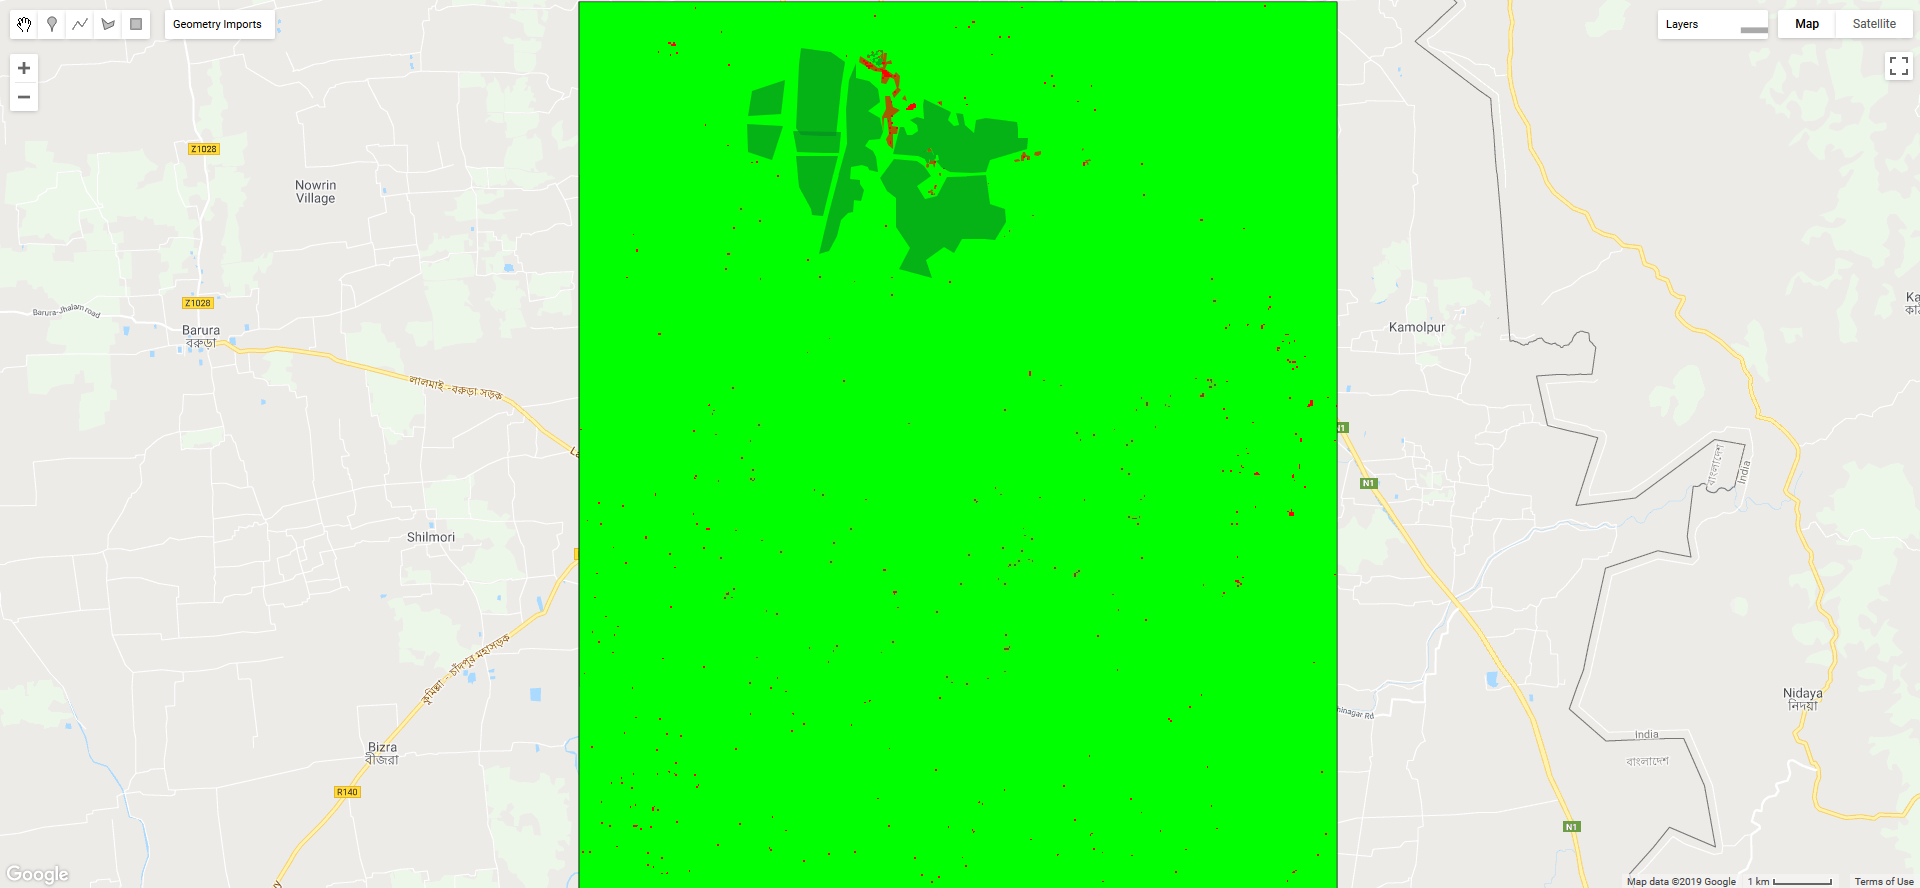
\includegraphics[width=\textwidth]{2001_ComillaSadaarDakshin}
\caption{Landsat 5 2001 Comilla Sadaar Dakshin}
\end{figure}

\textbf{DATA FROM 2011:}

\textsc{Builtup Area: } \textit{0.8010 sq.km.}

\textsc{Non-Builtup Area: } \textit{205.2820 sq.km.}

\textsc{Total Area: } \textit{206.0830 sq.km.}

\begin{figure}[H]
\centering
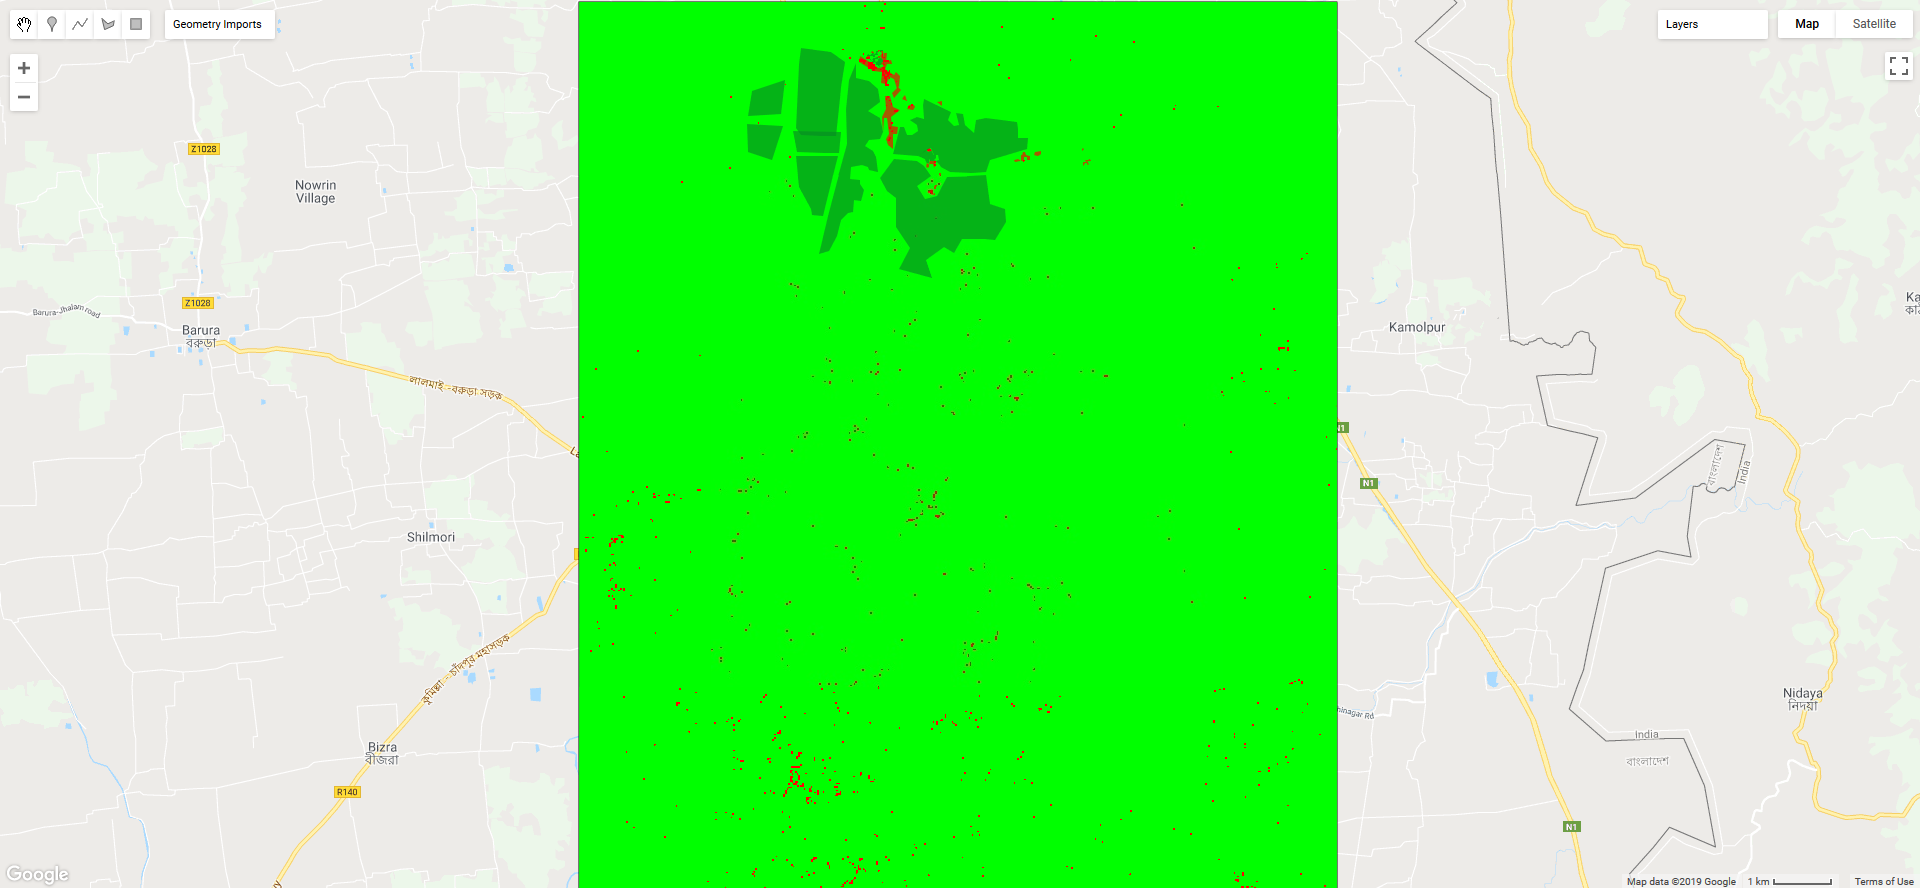
\includegraphics[width=\textwidth]{2011_ComillaSadaarDakshin}
\caption{Landsat 5 2011 Comilla Sadaar Dakshin}
\end{figure}

\vfill

The result obtained by the program using \textsf{Landsat 7} are given below:

\textbf{DATA FROM 2001:}

\textsc{Builtup Area: } \textit{0.5815 sq.km.}

\textsc{Non-Builtup Area: } \textit{205.5014 sq.km.}

\textsc{Total Area: } \textit{206.0830 sq.km.}

\begin{figure}[H]
\centering
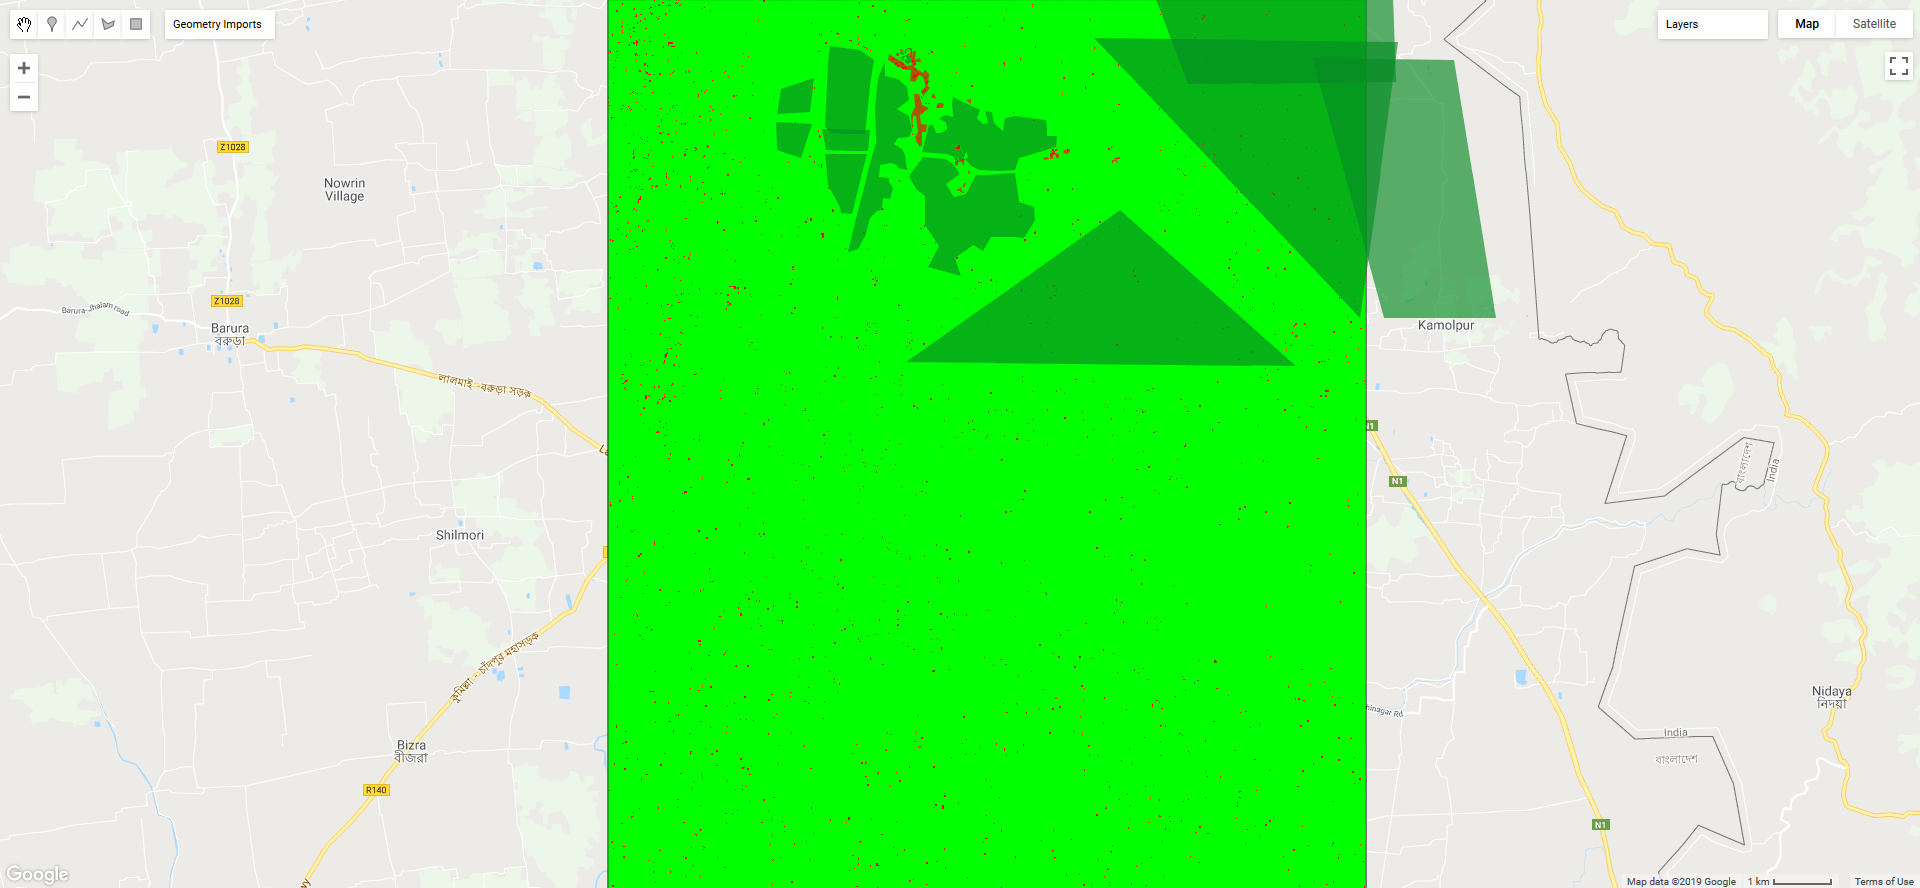
\includegraphics[width=\textwidth]{2001_ComillaSadaarDakshin_L7}
\caption{Landsat 7 2001 Comilla Sadaar Dakshin}
\end{figure}

\textbf{DATA FROM 2011:}

\textsc{Builtup Area: } \textit{0.7454 sq.km.}

\textsc{Non-Builtup Area: } \textit{147.5886 sq.km.}

\textsc{Total Area: } \textit{148.3341 sq.km.}

\begin{figure}[H]
\centering
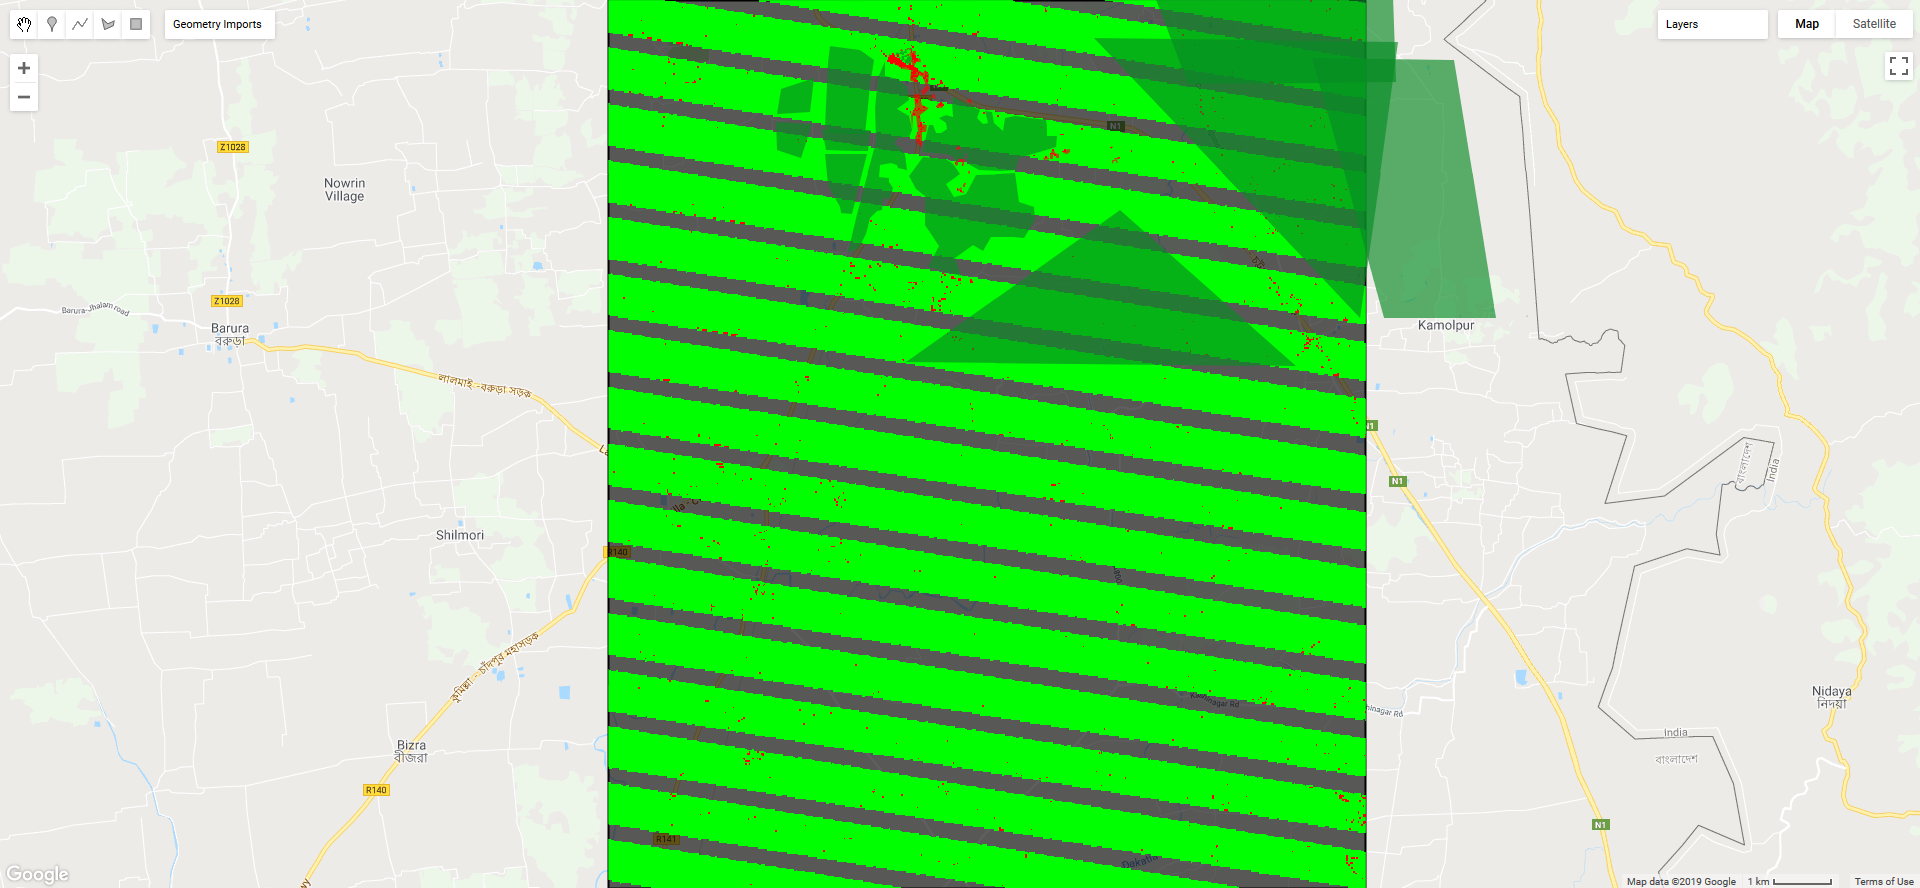
\includegraphics[width=\textwidth]{2011_ComillaSadaarDakshin_L7}
\caption{Landsat 7 2011 Comilla Sadaar Dakshin}
\end{figure}

Look at the figure 4, there are some blank stripes which makes the image unusable for area calculation, it is clearly reflected in the difference of total area of the both years.

\section{Mundumala}
Mundumala is an urban area which is just west to Tanore, Rajshahi. The left extremity of the urban area is 24.61\degree N, 88.46\degree E and the right extremity is 24.60\degree N, 88.46\degree E.

The result obtained by the program using \textsf{Landsat 5} are given below:

\textbf{DATA FROM 2001:}

\textsc{Builtup Area: } \textit{0.2079 sq.km.}

\textsc{Non-Builtup Area: } \textit{2.0353 sq.km.}

\textsc{Total Area: } \textit{2.2432 sq.km.}

\begin{figure}[H]
\centering
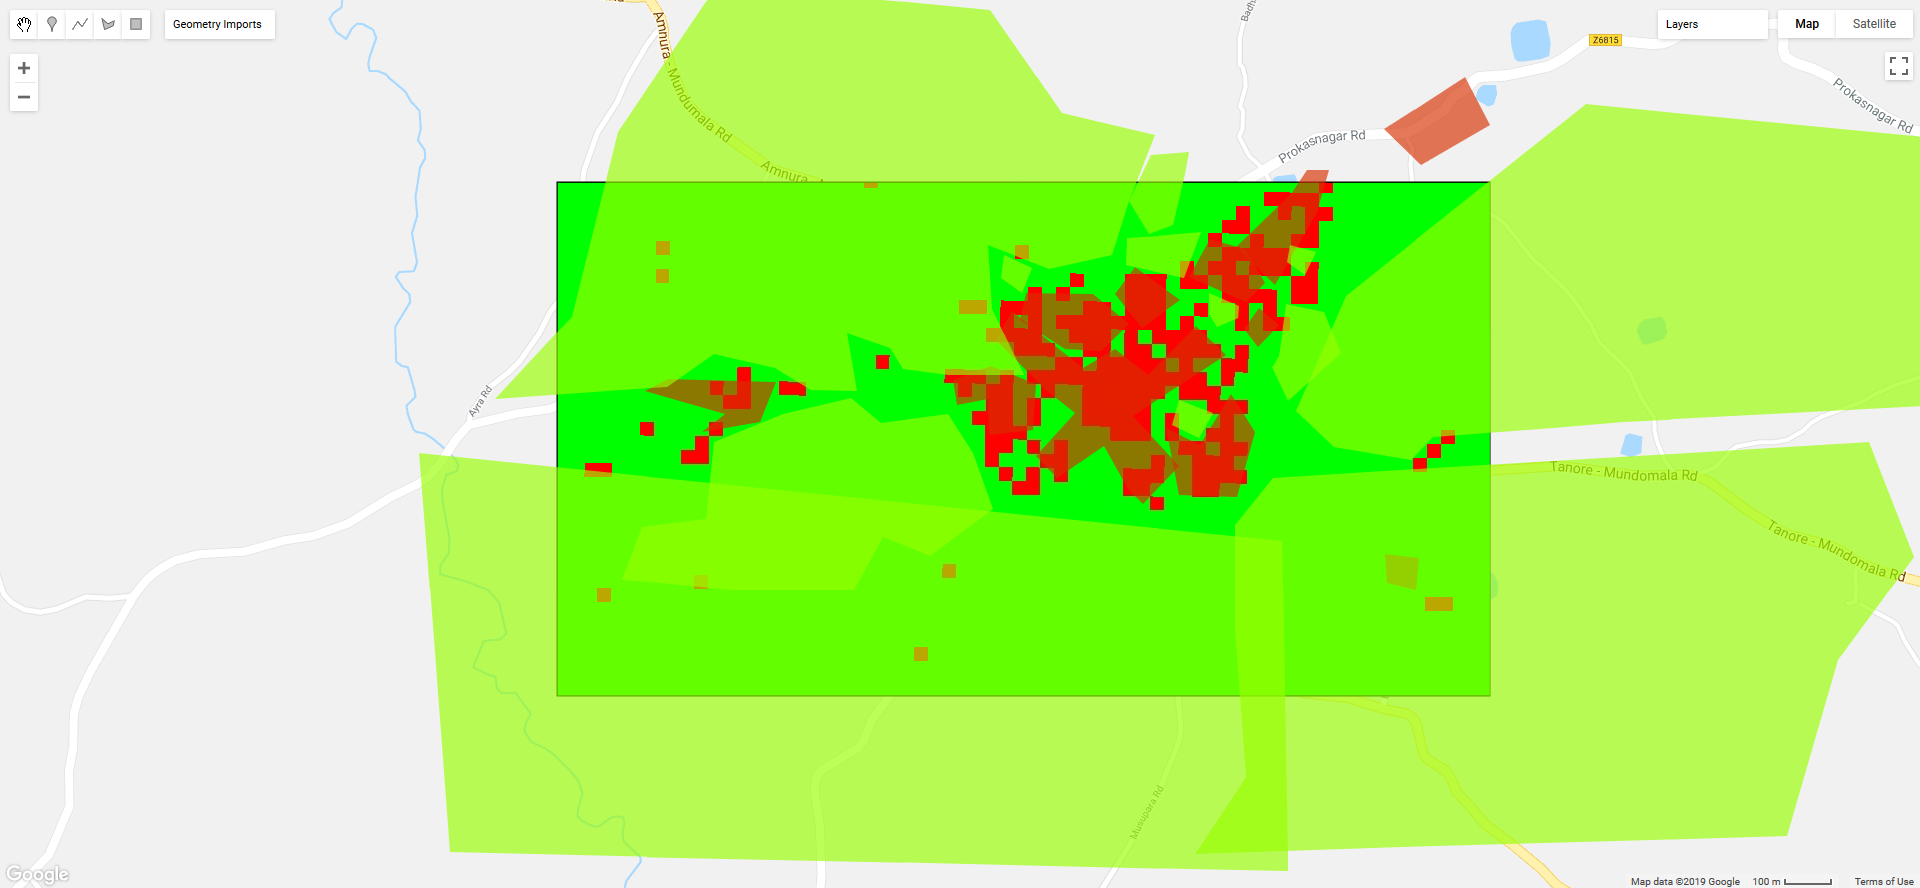
\includegraphics[width=\textwidth]{2001_Mundumala}
\caption{Landsat 5 2001 Mundumala}
\end{figure}

\textbf{DATA FROM 2011:}

\textsc{Builtup Area: } \textit{0.2809 sq.km.}

\textsc{Non-Builtup Area: } \textit{1.9623 sq.km.}

\textsc{Total Area: } \textit{2.2432 sq.km.}

\begin{figure}[H]
\centering
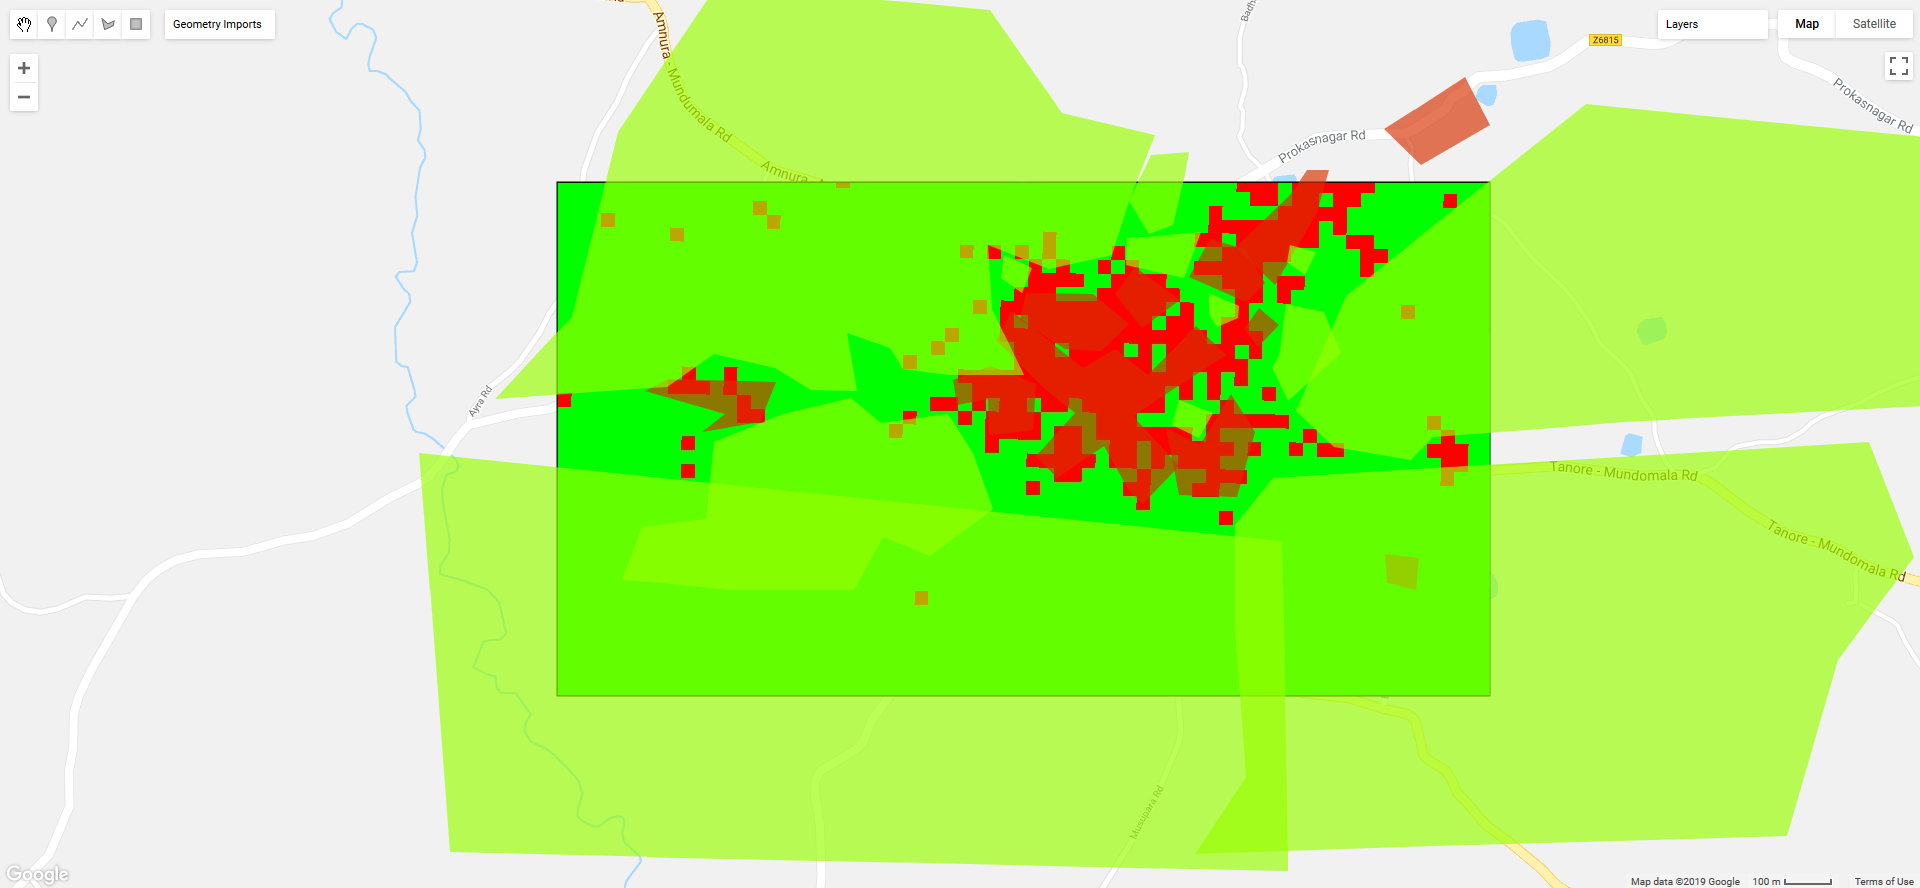
\includegraphics[width=\textwidth]{2011_Mundumala}
\caption{Landsat 5 2011 Mundumala}
\end{figure}

\vfill

The result obtained by the program using \textsf{Landsat 7} are given below:

\textbf{DATA FROM 2001:}

\textsc{Builtup Area: } \textit{0.2852 sq.km.}

\textsc{Non-Builtup Area: } \textit{1.9580 sq.km.}

\textsc{Total Area: } \textit{2.2432 sq.km.}

\begin{figure}[H]
\centering
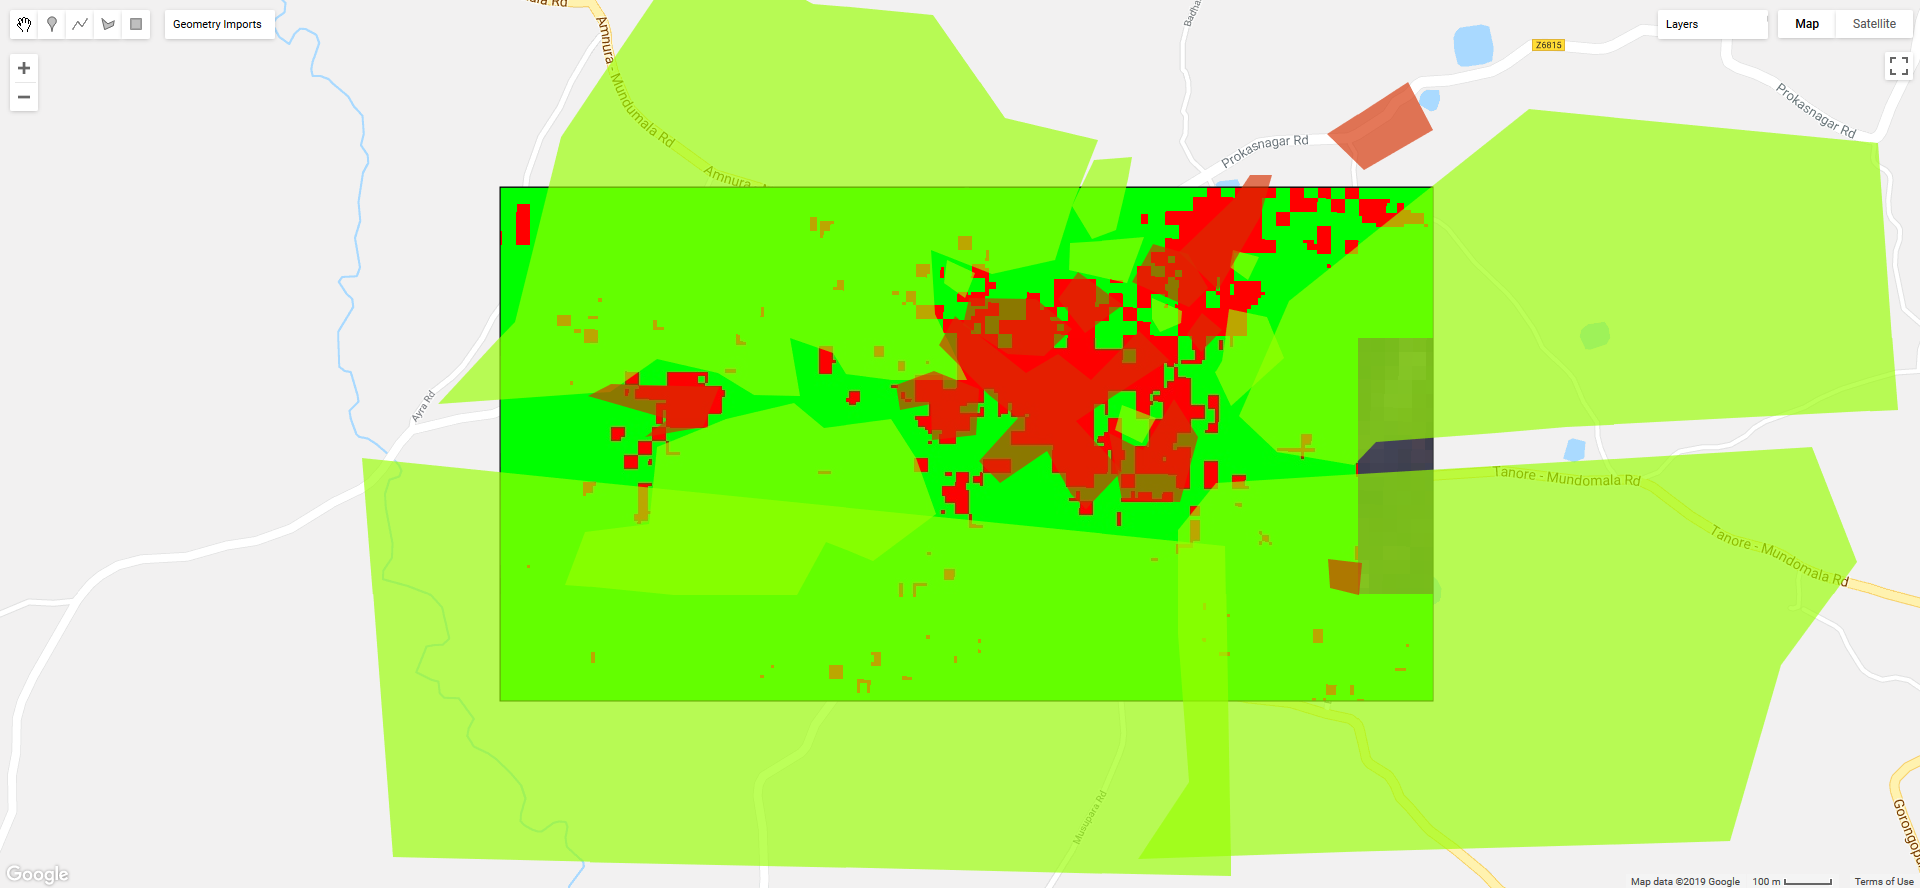
\includegraphics[width=\textwidth]{2001_Mundumala_L7}
\caption{Landsat 7 2001 Mundumala}
\end{figure}

\textbf{DATA FROM 2011:}

\textsc{Builtup Area: } \textit{0.2954 sq.km.}

\textsc{Non-Builtup Area: } \textit{1.3802 sq.km.}

\textsc{Total Area: } \textit{1.6757 sq.km.}

\begin{figure}[H]
\centering
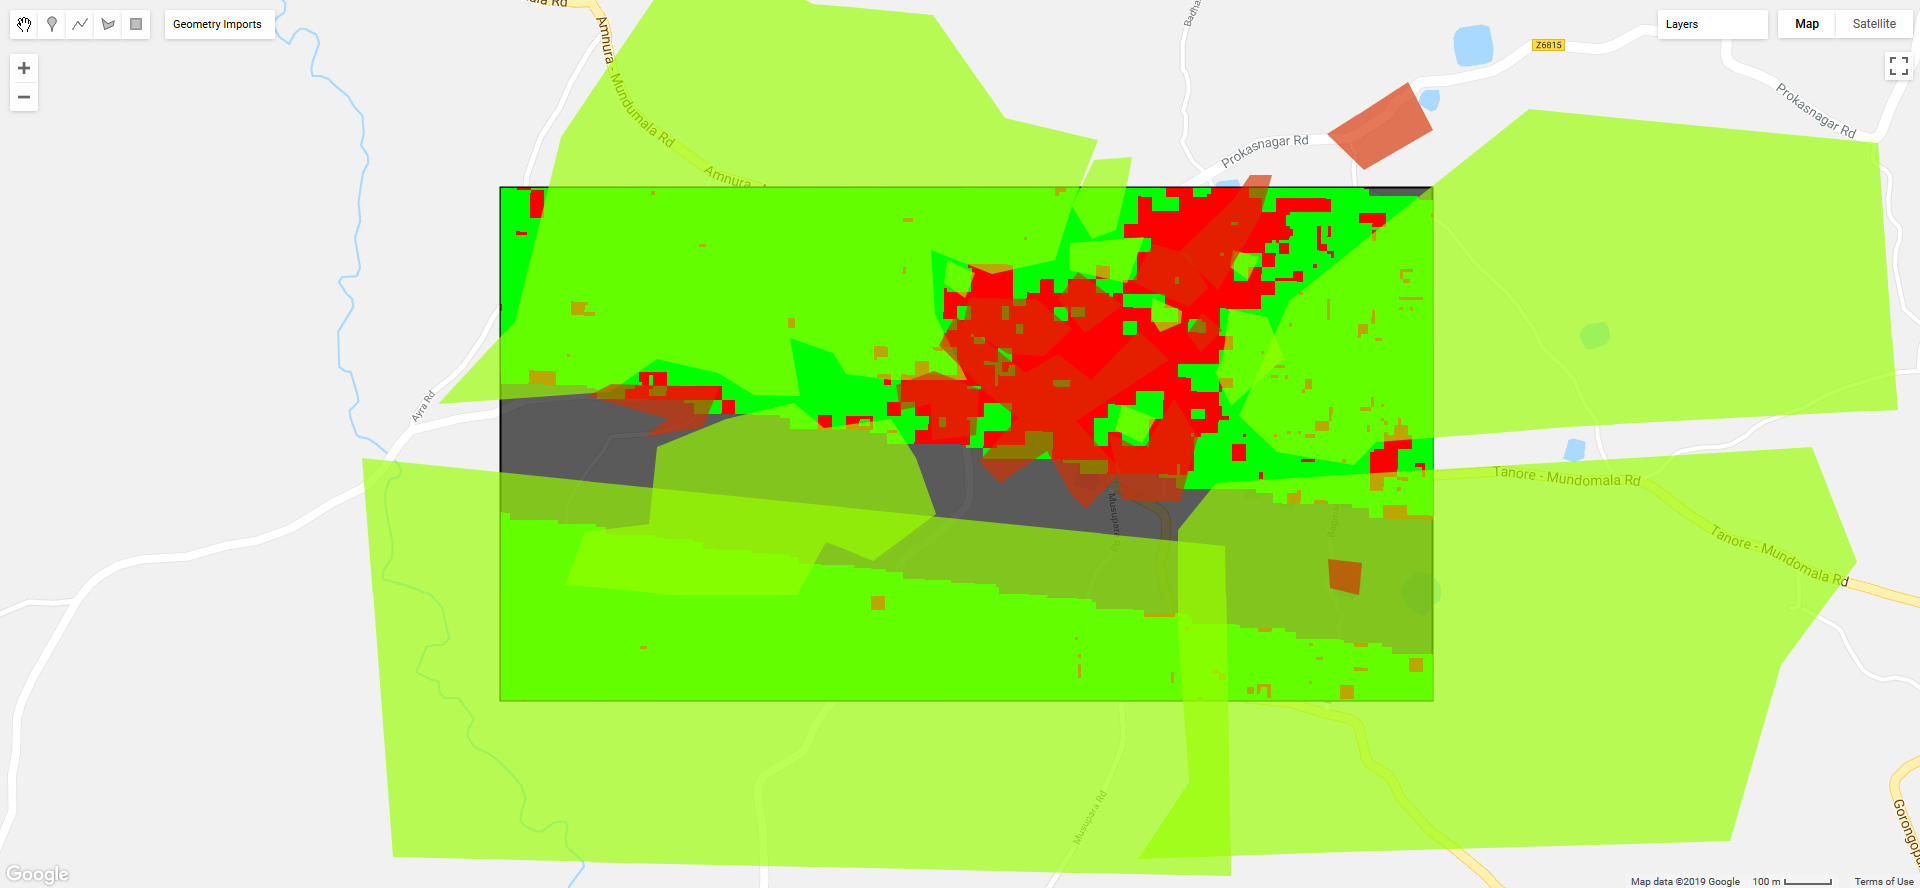
\includegraphics[width=\textwidth]{2011_Mundumala_L7}
\caption{Landsat 7 2011 Mundumala}
\end{figure}

The case is same as before here, the difference of area in the years states the unreliability of the Landsat 7 data.

\section{Hatiya}
Hatiya is the southern region, near Feni. It is small island created y silt, due to the change in the Padma's stream, it is slowing losing land. The left extremity of the urban area is 22.39\degree N, 91.04\degree E and the right extremity is 22.08\degree N, 91.19\degree E.

The result obtained by the program using \textsf{Landsat 7} are given below:

\textbf{DATA FROM 2001:}

\textsc{Builtup Area: } \textit{0 sq.km.}

\textsc{Non-Builtup Area: } \textit{278.8567 sq.km.}

\textsc{Total Area: } \textit{278.8567 sq.km.}

\begin{figure}[H]
\centering
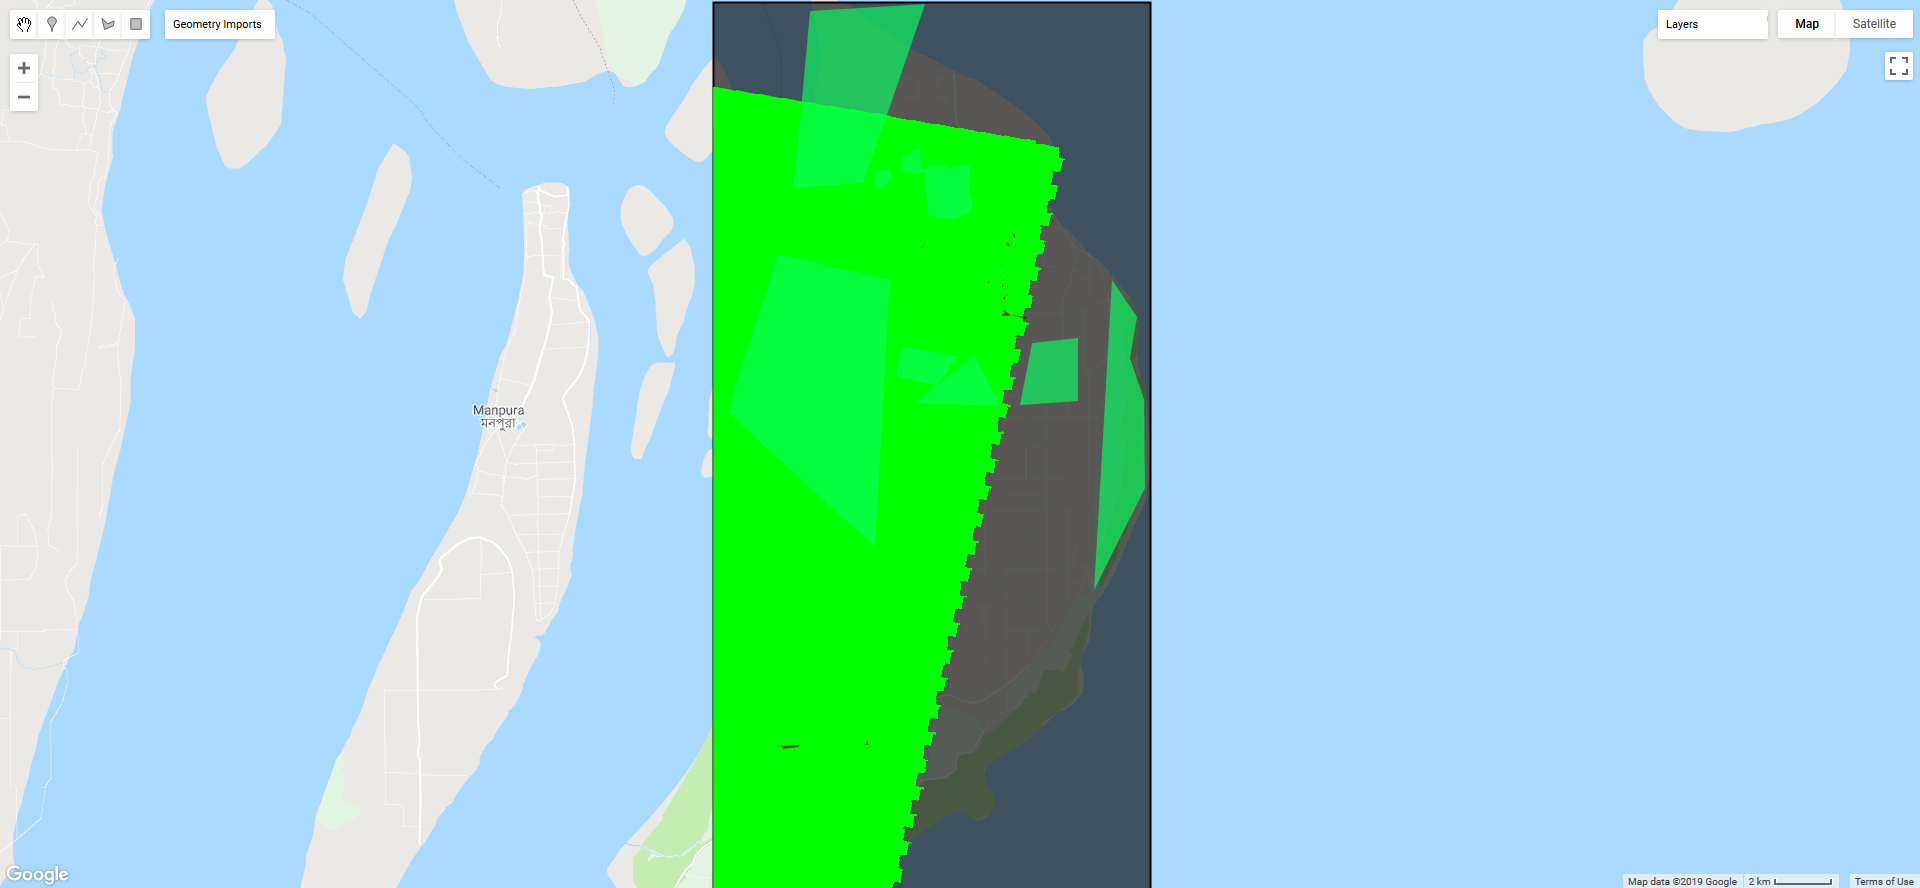
\includegraphics[width=\textwidth]{2001_Hatiya_L7}
\caption{Landsat 7 2001 Hatiya}
\end{figure}

\textbf{DATA FROM 2011:}

\textsc{Builtup Area: } \textit{1.5348 sq.km.}

\textsc{Non-Builtup Area: } \textit{399.8724 sq.km.}

\textsc{Total Area: } \textit{401.4072 sq.km.}

\begin{figure}[H]
\centering
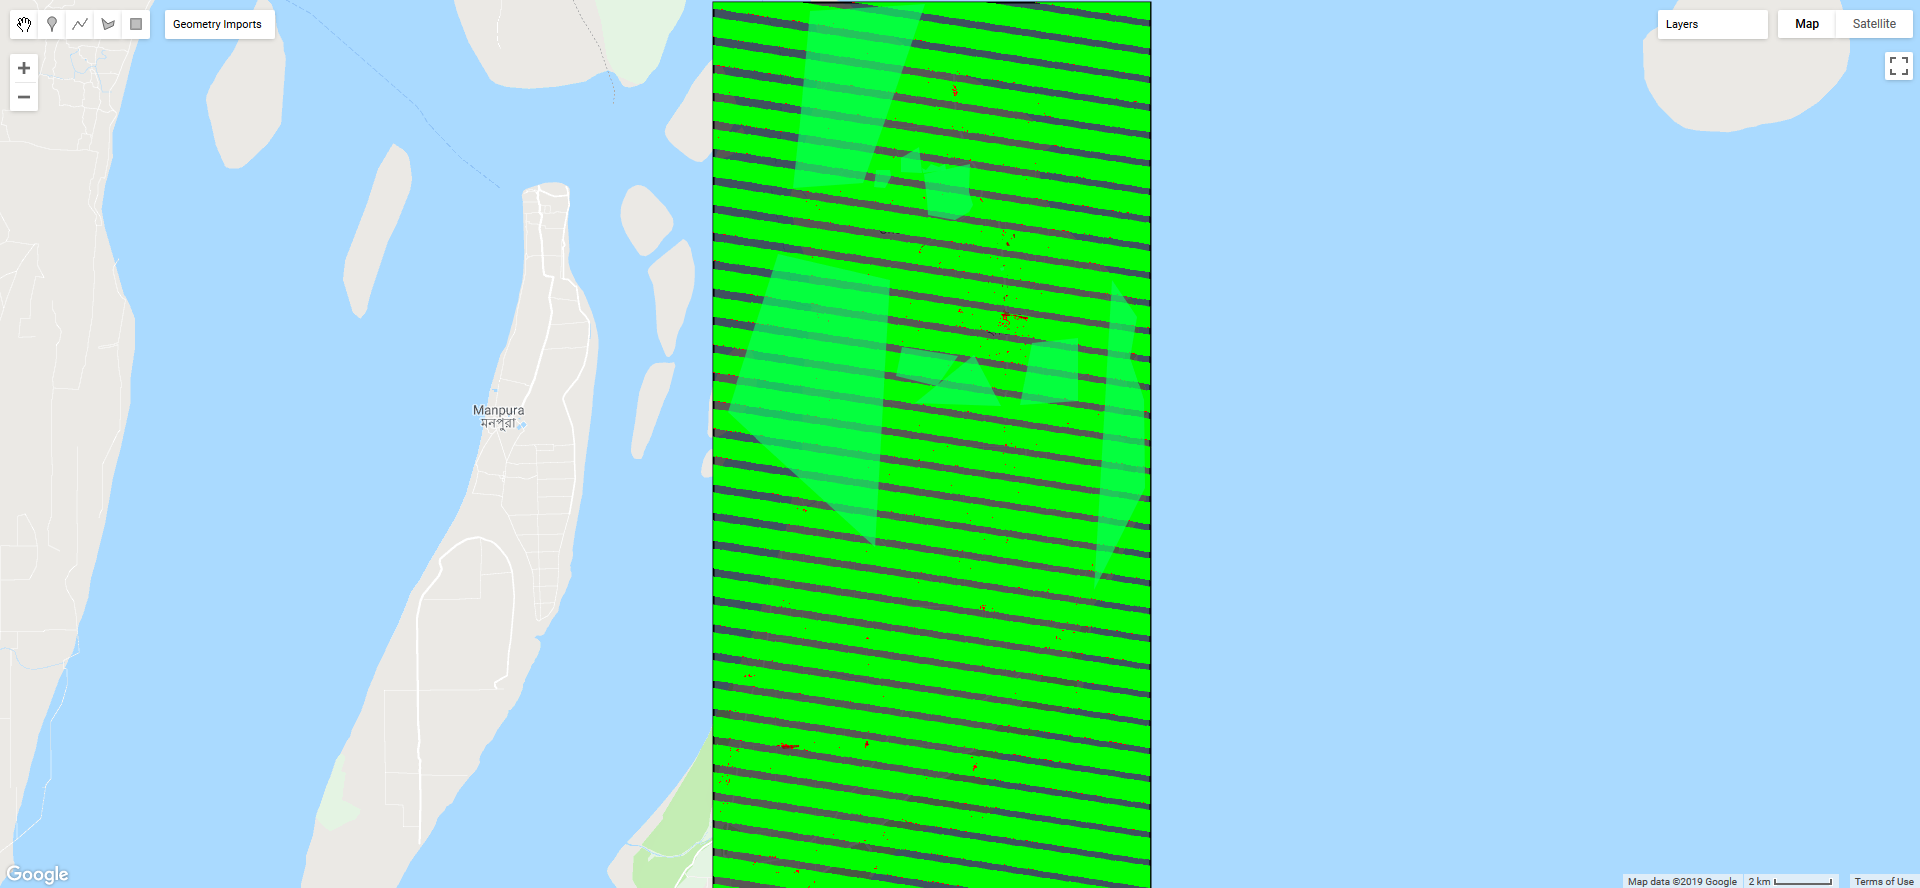
\includegraphics[width=\textwidth]{2011_Hatiya_L7}
\caption{Landsat 7 2011 Hatiya}
\end{figure}

Even though, the Landsat 7 data is inconsistent, I had to work with this because of the unavailability of any other data.
\vfill

\section{Conclusion}
From this research we can conclude that there was atleast 2 times increase of builtup in the urban areas, and the non-builtup area shrinked.

\end{document}